% 10‑Minute Beamer Deck: Complex Networks of ChatGPT Conversations
\documentclass[nodes]{beamer}
\usepackage[utf8]{inputenc}
\usepackage{graphicx}
\usepackage{pgfpages}
\setbeameroption{show notes on second screen=right}
\graphicspath{{./images/}}
\usepackage{booktabs}
\usepackage{tikz}
\usepackage{fontawesome5}
\usepackage{amsmath} % Needed for math formulas
\usetheme{Madrid}

%---------------------------------------------
% Meta
%---------------------------------------------
\title[ChatGPT Conversation Graph]{Cognitive MRI of ChatGPT Conversations}
\subtitle{Revealing the Hidden Structure of AI Conversations}
\author[Alex Towell]{Alex Towell \\ Southern Illinois University-Edwardsville \\
  \texttt{atowell@siue.edu} \\
  \texttt{lex@metafunctor.com}}
\date{\today}

\begin{document}

%------------------------------------------------
% 0. Title Slide (~30s)
%------------------------------------------------
\begin{frame}[plain]
  \titlepage
  \vspace{0.3cm}
  \centering\small
  Code: \href{https://github.com/queelius/chatgpt-complex-net}{github.com/queelius/chatgpt-complex-net}
  \note{
    \begin{itemize}
      \item Introduce: Research on analyzing ChatGPT conversations with network methods
      \item Key concept: "Cognitive MRI" - revealing hidden structures in conversation data
      \item This combines network science with modern language models
      \item (Transition) Let me explain why this matters...
    \end{itemize}
  }
\end{frame}

\begin{frame}{Why a Cognitive MRI?}
  \begin{itemize}
    \item Thousands of ChatGPT sessions $\rightarrow$ \alert{knowledge brain}.
    \item Raw logs are linear; \alert{neural (network) structure is hidden}.
    \item How can we visualize and analyze the relationships between conversations?
    \item Goal: Perform a \emph{cognitive MRI} of knowledge space:
      \begin{itemize}
        \item Reveal hidden \textbf{communities} (\alert{knowledge domains})
        \item Identify \textbf{bridge} conversations that connect domains (\alert{neural pathways})
        \item Map \textbf{semantic constraints} shaping network topology
      \end{itemize}
    \item Network science provides tools to make the invisible structure visible.
  \end{itemize}
  \begin{center}
    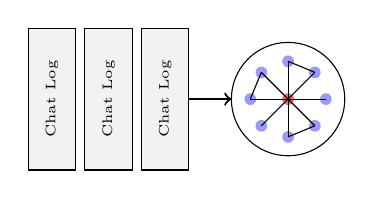
\begin{tikzpicture}[scale=0.6]
      \draw[fill=gray!10] (0,0) rectangle (1,3);
      \draw[fill=gray!10] (1.2,0) rectangle (2.2,3);
      \draw[fill=gray!10] (2.4,0) rectangle (3.4,3);
      % Linear logs
      \node[rotate=90] at (0.5,1.5) {\tiny Chat Log};
      \node[rotate=90] at (1.7,1.5) {\tiny Chat Log};
      \node[rotate=90] at (2.9,1.5) {\tiny Chat Log};
      \draw[->,thick] (3.4,1.5) -- (4.3,1.5);
      % Network
      \draw (5.5,1.5) circle (1.2);
      \foreach \i in {1,...,8} {
        \node[circle,fill=blue!40,inner sep=1.5pt] at ({5.5+cos(\i*45)*0.8},{1.5+sin(\i*45)*0.8}) {};
      }
      \node[circle,fill=red!60,inner sep=1.5pt] at (5.5,1.5) {};
      \foreach \i in {1,...,8} {
        \draw (5.5,1.5) -- ({5.5+cos(\i*45)*0.8},{1.5+sin(\i*45)*0.8});
      }
      \draw ({5.5+cos(45)*0.8},{1.5+sin(45)*0.8}) -- ({5.5+cos(90)*0.8},{1.5+sin(90)*0.8});
      \draw ({5.5+cos(135)*0.8},{1.5+sin(135)*0.8}) -- ({5.5+cos(180)*0.8},{1.5+sin(180)*0.8});
      \draw ({5.5+cos(270)*0.8},{1.5+sin(270)*0.8}) -- ({5.5+cos(315)*0.8},{1.5+sin(315)*0.8});
    \end{tikzpicture}
  \end{center}

  \note{
    \begin{itemize}
      \item Personal context: Generated 1000+ ChatGPT conversations over 18 months
      \item Problem: Linear archive with no organization or visible connections
      \item Goal: Transform flat data into structured knowledge map
      \item MRI analogy: Just as medical imaging reveals hidden structures in tissue
      \item Looking for: communities (domains), bridges (pathways), constraints
      \item (Point to diagram) From linear logs to organized network
      \item (Transition) First step: convert text to vectors...
    \end{itemize}
  }
\end{frame}


%------------------------------------------------
% 2. From Logs to Vectors (~1.5 min)
%------------------------------------------------
\begin{frame}{Representing Conversations as Vectors}
  How do we quantify the "meaning" of a conversation?
  \begin{columns}[T]
    \begin{column}{0.75\textwidth}
      \begin{itemize}
        \item \textbf{Old approach (e.g., Bag-of-Words):} Count keywords. Misses context.
        \item \textbf{Modern approach: Semantic Embeddings:} Use deep learning models (\texttt{nomic-embed-text}) to create vectors capturing semantics.
        \item \textbf{Process:}
          \begin{enumerate}
            \item Embed each user and assistant turn separately.
            \item Calculate mean embedding for user and assistant turns ($\vec e_u$ and $\vec e_a$).
            \item Weighted combo (user drives conversation):
              \[ \vec{e}_{\text{conv}} = \frac{2 \times \vec{e}_{u} + \vec{e}_{a}}{\lVert 2 \times \vec{e}_{u} + \vec{e}_{a} \rVert} \]
          \end{enumerate}
        \item Result: Each conversation is a point in a high-dimensional semantic space.
      \end{itemize}
    \end{column}
    \begin{column}{0.25\textwidth}
      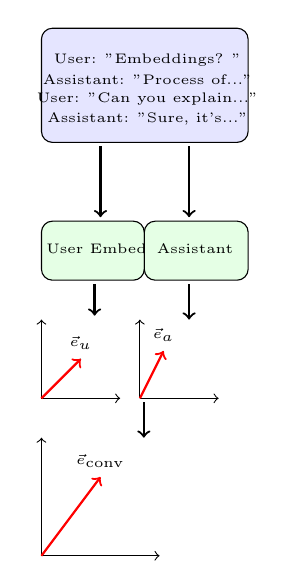
\begin{tikzpicture}[scale=0.5]
        % Conversation text
        \draw[rounded corners, fill=blue!10] (0,6.5) rectangle (5.25,9.4);
        \node at (2.7,8.6) {\tiny User: "Embeddings? "};
        \node at (2.7,8.1) {\tiny Assistant: "Process of..."};
        \node at (2.7,7.6) {\tiny User: "Can you explain..."};
        \node at (2.7,7.1) {\tiny Assistant: "Sure, it's..."};
        
        % Arrow to User
        \draw[->, thick] (1.5,6.4) -- (1.5,4.6);

        % Arrow to Assistant
        \draw[->, thick] (3.75,6.4) -- (3.75,4.6);

        % Embedding process
        \draw[rounded corners, fill=green!10] (0,3) rectangle (2.6125,4.5);
        \node at (1.4,3.8) {\tiny User Embed};
        
        % User embed
        \draw[rounded corners, fill=green!10] (2.6125,3) rectangle (5.25,4.5);
        \node at (3.9,3.8) {\tiny Assistant};

        % Arrow to vector space
        \draw[->, thick] (1.35,2.9) -- (1.35,2.1);

        % Embedding for user
        \draw[->] (0,0) -- (0,2);
        \draw[->] (0,0) -- (2,0);
        \draw[dashed] (0,0) -- (1,1) node[above] {\tiny $\vec{e}_{u}$};
        \draw[thick, red, ->] (0,0) -- (1,1);

        % Arrow to vector space
        \draw[->, thick] (3.75,2.9) -- (3.75,2);

        % Embedding for assistant
        \draw[->] (2.5,0) -- (2.5,2);
        \draw[->] (2.5,0) -- (4.5,0);
        \draw[dashed] (2.5,0) -- (3.1,1.2) node[above] {\tiny $\vec{e}_{a}$};
        \draw[thick, red, ->] (2.5,0) -- (3.1,1.2);
        

        % Arrow to vector space
        \draw[->, thick] (2.6,-0.1) -- (2.6,-1);
       
        % Vector space (coordinate system)
        \draw[->] (0,-4) -- (0,-1);
        \draw[->] (0,-4) -- (3,-4);
        \draw[dashed] (0,-4) -- (1.5,-2) node[above] {\tiny $\vec{e}_{\rm{conv}}$};
        \draw[thick, red, ->] (0,-4) -- (1.5,-2);
      \end{tikzpicture}
    \end{column}
  \end{columns}
  \note{
  \begin{itemize}
    \item Challenge: Making "meaning" mathematically analyzable
    \item Traditional methods (bag-of-words): Just keyword counting, loses context
    \item Modern approach: Neural embeddings capture semantic meaning
    \item Process: (point to diagram)
      \begin{itemize}
        \item Split by speaker role
        \item User turns weighted 2x (they drive conversation direction)
        \item Result: Each conversation = point in high-dim semantic space
      \end{itemize}
    \item (Transition) Now we build connections between these points...
  \end{itemize}
    }
\end{frame}

\begin{frame}{Building the Semantic Network}
  From vectors to a network:
  \begin{columns}[T]
    \begin{column}{0.65\textwidth}
      \begin{enumerate}
        \item \textbf{Nodes:} Each conversation becomes a node.
        \item \textbf{Links:} Link conversations based on similarity.
          \[ \text{sim}(\vec{e}_i, \vec{e}_j) = \frac{\vec{e}_i \cdot \vec{e}_j}{\lVert \vec{e}_i \rVert \lVert \vec{e}_j \rVert} \]
        \item \textbf{Threshold:} Keep only strong connections ($\geq 0.9$).
        \item \textbf{Focus:} Analyze Giant Component.
      \end{enumerate}
    \end{column}
    \begin{column}{0.35\textwidth}
      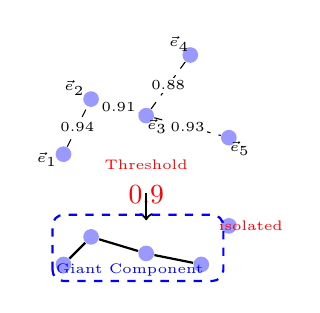
\begin{tikzpicture}[scale=0.7]
        % Vector points in semantic space
        \node[circle, fill=blue!40, inner sep=2pt] (a) at (0,0) {};
        \node[circle, fill=blue!40, inner sep=2pt] (b) at (0.5,1) {};
        \node[circle, fill=blue!40, inner sep=2pt] (c) at (1.5,0.7) {};
        \node[circle, fill=blue!40, inner sep=2pt] (d) at (2.3,1.8) {};
        \node[circle, fill=blue!40, inner sep=2pt] (e) at (3,0.3) {};
        
        % Labels for vector points
        \node at (-0.3,-0.1) {\tiny $\vec{e}_1$};
        \node at (0.2,1.2) {\tiny $\vec{e}_2$};
        \node at (1.7,0.5) {\tiny $\vec{e}_3$};
        \node at (2.1,2) {\tiny $\vec{e}_4$};
        \node at (3.2,0.1) {\tiny $\vec{e}_5$};
        
        % Draw similarity measurements with values
        \draw[dashed] (a) -- node[fill=white,inner sep=1pt] {\tiny 0.94} (b);
        \draw[dashed] (b) -- node[fill=white,inner sep=1pt] {\tiny 0.91} (c);
        \draw[dashed] (c) -- node[fill=white,inner sep=1pt] {\tiny 0.88} (d);
        \draw[dashed] (c) -- node[fill=white,inner sep=1pt] {\tiny 0.93} (e);
        
        % Threshold label
        \node[red, align=center] at (1.5,-0.5) {\tiny Threshold\\0.9};
        \draw[->, thick] (1.5,-0.7) -- (1.5,-1.2);
        
        % Network after thresholding - simpler layout
        \node[circle, fill=blue!40, inner sep=2pt] (a2) at (0,-2) {};
        \node[circle, fill=blue!40, inner sep=2pt] (b2) at (0.5,-1.5) {};
        \node[circle, fill=blue!40, inner sep=2pt] (c2) at (1.5,-1.8) {};
        \node[circle, fill=blue!40, inner sep=2pt] (e2) at (2.5,-2) {};
        \node[circle, fill=blue!40, inner sep=2pt] (d2) at (3,-1.3) {};
        
        % Draw edges that passed threshold
        \draw[thick] (a2) -- (b2);
        \draw[thick] (b2) -- (c2);
        \draw[thick] (c2) -- (e2);
        
        % Label isolated node
        \node[red] at (3.4,-1.3) {\tiny isolated};
        
        % Giant component with clearer boundary
        \draw[blue, thick, dashed, rounded corners] (-0.2,-2.3) rectangle (2.9,-1.1);
        \node[blue] at (1.2,-2.1) {\tiny Giant Component};
      \end{tikzpicture}    \end{column}
  \end{columns}
  \vspace{0.2cm}
  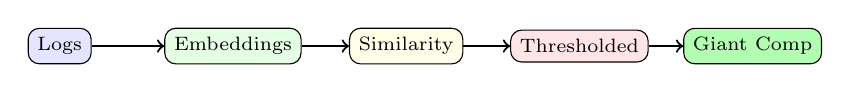
\begin{tikzpicture}[node distance=2.2cm, every node/.style={font=\scriptsize}]
    \node[draw, rounded corners, fill=blue!10] (logs) {Logs};
    \node[draw, rounded corners, fill=green!10, right of=logs] (embed) {Embeddings};
    \node[draw, rounded corners, fill=yellow!10, right of=embed] (sim) {Similarity};
    \node[draw, rounded corners, fill=red!10, right of=sim] (graph) {Thresholded};
    \node[draw, rounded corners, fill=green!30, right of=graph] (giant) {Giant Comp};
    \draw[->, thick] (logs) -- (embed);
    \draw[->, thick] (embed) -- (sim);
    \draw[->, thick] (sim) -- (graph);
    \draw[->, thick] (graph) -- (giant);
  \end{tikzpicture}
\end{frame}

\note{
  \begin{itemize}
    \item Network construction process: [point to each step]
    \begin{enumerate}
      \item Nodes = conversations
      \item Links = similarity above threshold (cosine similarity)
      \item High threshold (0.9) keeps only strong connections
      \item Focus on giant component for analysis
    \end{enumerate}
    \item (Point to visualization) Shows filtering process
    \item Similar to contrast enhancement in medical imaging
    \item 449 conversations in giant component (about half of dataset)
    \item (Transition) Let's see what this network looks like...
  \end{itemize}
}

%------------------------------------------------
% 4. Network Snapshot (~1 min)
%------------------------------------------------
\begin{frame}{The Conversation Network}
  \begin{columns}[T]
    \begin{column}{0.35\textwidth}
      \scriptsize
      \textbf{Giant Component (0.9 Threshold):}
      \vspace{0.1cm}
      \begin{tabular*}{\linewidth}{@{\extracolsep{\fill}} lr}
        \toprule
        Nodes ($|N|$)         & 449 \\
        Links ($|L|$)         & 1615 \\
        Avg. Degree           & 7.2 \\
        Clustering ($C$)      & 0.60 \\
        Path Length ($\ell$)  & 5.8 \\
        Diameter              & 18 \\
        Modularity ($Q$)      & 0.75 \\
        \bottomrule
      \end{tabular*}
      \vspace{0.2cm}
      \begin{itemize}
        \item High clustering (0.60) → \alert{Strong local neighborhoods}
        \item High modularity (0.75) → \alert{Clear community structure}
        \item Small average path length (5.8) → \alert{Navigable topology}
      \end{itemize}
    \end{column}
    \begin{column}{0.65\textwidth}
      \includegraphics[width=\linewidth]{images/cluster-vis.png}
    \end{column}
  \end{columns}
  \note{
    \begin{itemize}
    \item (Point to visualization) Clear clustering visible in different colors
    \item Key metrics tell us about structure: (point to metrics)
    \begin{itemize}
       \item High clustering (0.60): Strong local neighborhoods
       \item High modularity (0.75): Clear community boundaries
       \item Relatively short paths (5.8 steps): Knowledge is navigable
    \end{itemize}
    \item Notice varying density across regions - different knowledge organization
    \item (Transition) Let's identify these communities...
    \end{itemize}
  }
\end{frame}


%------------------------------------------------
% 5. Finding Thematic Communities (~1 min)
%------------------------------------------------
\begin{frame}{Finding Thematic Communities}
  \begin{columns}[T]
    \begin{column}{0.38\textwidth}
      \small
      \textbf{Community Detection:}
      \begin{itemize}
        \item $\sim$ 15 communities
        \item \scriptsize (High) modularity score: 0.75
      \end{itemize}
      \vspace{0.1cm}
      \textbf{Major Knowledge Domains:}
      \scriptsize
      \begin{enumerate}
          \item \textcolor{blue}{ML/AI/LLM} \tiny(23\%)
          \item \textcolor{green}{Statistics \& Probability} \tiny(18\%) 
          \item \textcolor{orange}{M.S. Math/Analysis} \tiny(14\%)
          \item \textcolor{red}{Philosophy \& AI Ethics} \tiny(10\%)
          \item \textcolor{cyan}{Programming Projects} \tiny(10\%)
          \item \textcolor{purple}{Programming/Algorithms} \tiny(7\%)
      \end{enumerate}
      \vspace{0.1cm}
      \small
      Distinct structural patterns across communities:
      \begin{itemize}
        \item \scriptsize Variable local clustering (0.40-0.58)
        \item \scriptsize Core-periphery vs. distributed topologies
      \end{itemize}
    \end{column}
    \begin{column}{0.62\textwidth}
      \includegraphics[width=\linewidth]{images/cluster-vis-topics-better.png}
    \end{column}
  \end{columns}
  \note{
    \begin{itemize}
    \item Used Louvain algorithm - found 15 communities
    \item [Point to colored communities list]
    \begin{itemize}
       \item Blue: ML/AI/LLM (23\%) - largest domain
       \item Green: Statistics (18\%)
       \item Orange: Advanced math (14\%)
       \item Others: Philosophy, programming, etc.
    \end{itemize}
    \item Different internal structures:
      \begin{itemize}
        \item AI/ML has hub-spoke pattern
        \item Programming projects more distributed
      \end{itemize}
    \item (Point to visualization) Colors match communities list
    \item (Transition) How robust are these findings?
    \end{itemize}
  }
\end{frame}

%------------------------------------------------
% 6. Threshold Sensitivity (~1 min)
%------------------------------------------------
\begin{frame}{Threshold Sensitivity: 0.9 vs 0.875}
  How robust is the structure to the similarity threshold?
  \begin{columns}[T]
    \begin{column}{0.55\textwidth}
      \includegraphics[width=\linewidth]{images/0.875-wild-better.png}
      \begin{center}
        \scriptsize Network at 0.875 threshold
      \end{center}      
    \end{column}
    \begin{column}{0.45\textwidth}
      \scriptsize
      \begin{tabular}{lcc}
        \toprule
        \textbf{Metric}    & \textbf{0.9} & \textbf{0.875} \\
        \midrule
        Nodes              & 449          & 825 \textcolor{red}{(+84\%)} \\
        Links              & 1615         & 5652 \textcolor{red}{(+250\%)} \\
        Avg. Degree        & 7.2          & 13.7          \\
        Avg. Path Len.     & 5.8          & 3.9           \\
        Diameter           & 18           & 12            \\
        Modularity         & 0.75         & 0.65          \\
        Clustering         & 0.60         & 0.60          \\
        \bottomrule
      \end{tabular}
      \vspace{0.1cm}
      \\ \textbf{Findings:}
      \begin{itemize}
          \item Network expands significantly but more navigable (shorter paths).
          \item \alert{Community structure persists} (high modularity) and local clustering stable.
          \item New communities appear (\textbf{niece})
      \end{itemize}
      \textbf{Conclusion:} 0.9 threshold provides clearer structure, but 0.875 reveals weaker links and validates robustness.
    \end{column}
  \end{columns}
\note{
  \begin{itemize}
  \item Testing robustness: Slightly lowered threshold (0.9 -> 0.875)
  \item (Point to numbers) Dramatic expansion: +84\% nodes, +250\% links
  \item (Point to key findings)
  \begin{itemize}
    \item Community structure persists despite expansion
    \item Clustering coefficient stays exactly 0.60
    \item New distinct communities appear (e.g., niece conversations)
  \end{itemize}
  \item Confirms findings aren't artifacts of arbitrary threshold
  \item (Transition) How do these knowledge domains connect?
  \end{itemize}
}  
\end{frame}

%------------------------------------------------
% 7. Bridging Knowledge Domains (~1 min)
%------------------------------------------------
\begin{frame}{Bridging Knowledge Domains}
  \textbf{How do different knowledge areas connect?} $\rightarrow$ \textbf{Betweenness Centrality} ($C_B$)
  \begin{columns}[T]
    \begin{column}{0.55\textwidth}
      \includegraphics[width=\linewidth]{images/bridge-better.png}
      \scriptsize \textbf{Zoomed view of bridge conversations connecting communities}
    \end{column}
    \begin{column}{0.45\textwidth}
      \scriptsize High $C_B$ nodes lie on many shortest paths between other nodes.\\
      \vspace{0.1cm}
      \textbf{Key Finding:} Multiple bridge types exist!
      \begin{tabular}{lrrl}
        \toprule
        \textbf{Conversation} & $\langle k \rangle$ & \textbf{$C_B$} & \textbf{Type} \\
        \midrule
        \scriptsize geometric-mean & 61 & 45k & Eolut. \\
        \scriptsize mcts-code & 10 & 37k & Integrative \\
        \scriptsize cuda-program & 2 & 9.8k & Pure \\
        \bottomrule
      \end{tabular}
      \vspace{0.2cm}
      \begin{itemize}
        \item \textbf{Evolutionary bridges:} High-degree nodes that expand across domains through topic drift
        \item \textbf{Integrative bridges:} Specialized nodes deliberately connecting distinct domains
        \item \textbf{Pure bridges:} Low-degree nodes that form critical links between specific communities
      \end{itemize}
    \end{column}
  \end{columns}
  \note{
  \begin{itemize}
    \item Betweenness centrality reveals bridges between communities
    \item (Point to visualization) Zoomed view of key bridges
    \item Discovered three bridge types: (point to table)
    \begin{itemize}
      \item Evolutionary bridges (geometric-mean): High degree \& betweenness
      \item Integrative bridges (mcts-code): Deliberate synthesis
      \item Pure bridges (cuda-program): Minimal connections but critical links
    \end{itemize}
    \item Different mechanisms for knowledge integration
    \item (Transition) Let's look at connectivity patterns...
  \end{itemize}
  }
\end{frame}

%------------------------------------------------
% 8. Network Structure: Degree Distribution (~1 min)
%------------------------------------------------
\begin{frame}{Network Structure: Degree Distribution}
  How connected are conversations?
  \begin{columns}[T]
    \begin{column}{0.5\textwidth}
      \includegraphics[width=\linewidth]{images/degree_distribution_histogram.pdf}
      \scriptsize \textbf{Most conversations have few connections}\\
      \scriptsize \textbf{A few hubs have many connections}
    \end{column}
    \begin{column}{0.5\textwidth}
      \begin{itemize}
          \item Strongly right-skewed distribution
          \item A few hub nodes link to 33\% of all conversations
          \item \alert{Partial scale-free properties}: Power-law fit ($\gamma \approx 4.7$) only applies to highest-degree nodes ($k \ge 20$)
          \item Deviates from Erdős-Rényi and pure scale-free models
          \item Semantic constraints limit hub growth -- we'll analyze this next.
      \end{itemize}
    \end{column}
  \end{columns}
  \note{
    \begin{itemize}
      \item (Point to histogram) Heavily skewed distribution
      \item Most conversations have few connections
      \item Few hubs connect to many others (one links to 14\% of network)
      \item Not purely scale-free: Power law only in tail (k>=20)
      \item Much steeper falloff than typical scale-free (gamma ~ 4.7 vs 2-3)
      \item Suggests semantic constraints limit hub growth
      \item (Transition) Is this just preferential attachment?
    \end{itemize}
  }
\end{frame}

%------------------------------------------------
% 9. Beyond Simple Network Growth (~1 min)
%------------------------------------------------
\begin{frame}{Beyond Simple Network Growth Models}
  Is this just \alert{preferential attachment} (rich get richer)?
  \begin{columns}[T]
    \begin{column}{0.45\textwidth}
      \includegraphics[width=\linewidth]{images/degree_overlay.png}
      \scriptsize \textbf{Degree distribution comparison}\\
      \scriptsize Conversation network vs. Barabási-Albert
    \end{column}
    \begin{column}{0.45\textwidth}
      \includegraphics[width=\linewidth]{images/metrics_boxplot.png}
      \scriptsize \textbf{Network properties comparison}\\
      \scriptsize Higher clustering, longer paths than BA
    \end{column}
  \end{columns}
  \vspace{0.1cm}
  \scriptsize \textbf{Key findings:}
  \begin{itemize}
    \item \scriptsize Steeper degree tail ($\gamma \approx 4.7$ vs. $\gamma = 3$) indicates \alert{constrained hub growth}
    \item \scriptsize Much higher clustering suggests \alert{topical organization}
    \item \scriptsize Longer paths reflect \alert{cognitive distance} between domains
  \end{itemize}
  \small \textbf{Conclusion:} Not just preferential attachment - semantic constraints / cognitive exploration patterns shape network structure.
  \note{
  \begin{itemize}
    \item Compared with Barabási-Albert preferential attachment model
    \item (Point to left graph) Much steeper degree falloff
    \item (Point to right graph) ~6x higher clustering than BA model
    \item Three key differences:
    \begin{itemize}
      \item Constrained hub growth (semantic limitations)
      \item Strong topical organization (high clustering)
      \item Meaningful distances between domains (longer paths)
    \end{itemize}
    \item Not just "rich get richer" - semantic constraints matter
    \item (Transition) Let's wrap up what we've learned...
  \end{itemize}
  }
\end{frame}

%------------------------------------------------
% 10. Application: Network-Aware Recommendations (~30s)
%------------------------------------------------
\begin{frame}{Application: Network-Aware Recommendations}
  \scriptsize If time permits - otherwise skip to conclusions
  \normalsize
  
  \begin{columns}[T]
    \begin{column}{0.6\textwidth}
      Score past conversations by balancing:
      \vspace{0.1cm}
      \[
        \rm{score}(c_i) = \alpha \times
          \underbrace{\rm{sim}(\vec e_{\rm{cur}}, \vec e_i)}_{\rm{Familiarity}} + \beta \times \underbrace{\widehat{C_B}(c_i)}_{\rm{Bridging}} 
      \]
      \vspace{0.1cm}
      \begin{itemize}
        \item \scriptsize $\alpha \gg \beta$: Favor similar conversations
        \item \scriptsize $\alpha \approx \beta$: Balance familiar with bridging 
        \item \scriptsize $\alpha \ll \beta$: Prioritize knowledge-connecting bridges
      \end{itemize}
    \end{column}
    \begin{column}{0.4\textwidth}
      \scriptsize \textbf{Example ($\alpha=2, \beta=1$):}
      \begin{itemize}
        \item High-sim conversations dominate top slots
        \item Bridge nodes (e.g., ``geometric-mean'') still appear mid-list
        \item Single parameter to control exploration vs. exploitation
      \end{itemize}
    \end{column}
  \end{columns}
  \note{
  \begin{itemize}
    \item Practical application: Recommendation system using network structure
    \item Formula balances: similarity vs. bridging potential
    \item Can tune parameters for exploration vs. exploitation
    \item (Skip if running behind schedule)
  \end{itemize}
  }
\end{frame}

%------------------------------------------------
% 11. Conclusions (~1 min)
%------------------------------------------------
\begin{frame}{Conclusions}
  \begin{columns}[T]
    \begin{column}{0.55\textwidth}
      \textbf{Key Findings:}
      \begin{itemize}
        \item Conversation archives reveal rich \alert{cognitive structure}
        \item Strong \alert{communities} align with knowledge domains
        \item Multiple \alert{bridge types} connect knowledge areas
        \item Structure suggests \alert{semantic constraints} beyond simple attachment
        \item Network structure enables applications like smart recommendations
      \end{itemize}
    \end{column}
    
    \begin{column}{0.45\textwidth}
      \begin{center}
        \includegraphics[width=0.7\linewidth]{images/cluster-vis-topics-better.png}
        \vspace{0.5cm}
        
        \textbf{Thank You!}
        \vspace{0.3cm}
        
        \scriptsize
        \faEnvelope~lex@metafunctor.com \\
        \vspace{0.1cm}
        \faGithub~\href{https://github.com/queelius/chatgpt-complex-net}{github.com/queelius/chatgpt-complex-net}
      \end{center}
    \end{column}
  \end{columns}
  
  \note{
  \begin{itemize}
  \item Key contributions:
  \begin{itemize}
    \item Network approach reveals cognitive structure in conversations
    \item Communities align with knowledge domains
    \item Multiple bridge types connect domains (evolutionary, integrative, pure)
    \item Evidence of semantic constraints beyond simple growth models
  \end{itemize}
  \item "Cognitive MRI" makes visible what was hidden in linear logs
  \item Code available on GitHub for reproducing analysis
  \item Thank you! Questions?
  \end{itemize}
 }
\end{frame}

\end{document}
